\documentclass[a4paper]{ctexart}
	\usepackage{pgf,tikz}
	\thispagestyle{empty}
\begin{document}
	\begin{center}
		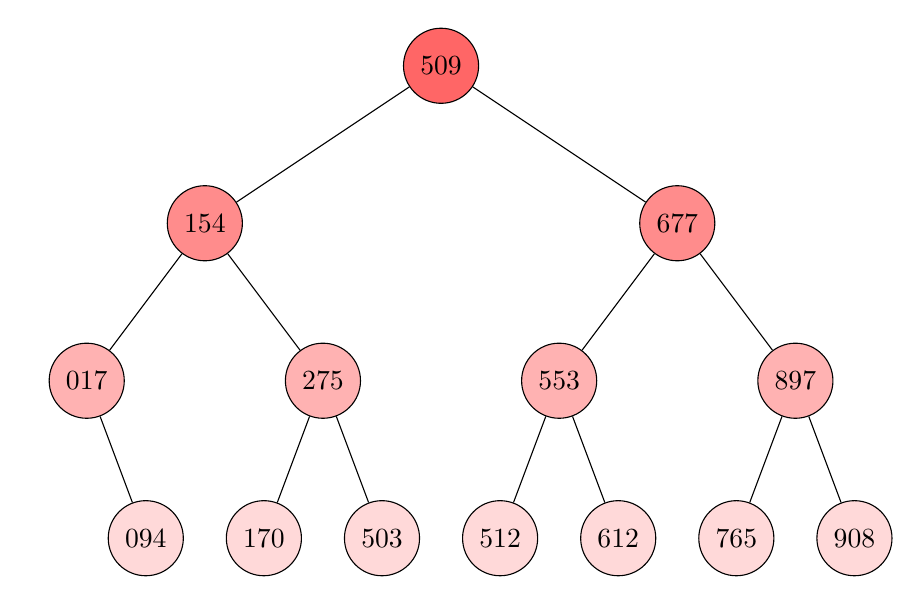
\begin{tikzpicture}[level distance=20mm] 
			\tikzstyle{every node}=[fill=red!60,circle,inner sep=4pt] 
			\tikzstyle{level 1}=[sibling distance=60mm, 
				set style={{every node}+=[fill=red!45]}] 
			\tikzstyle{level 2}=[sibling distance=30mm, 
				set style={{every node}+=[fill=red!30]}] 
			\tikzstyle{level 3}=[sibling distance=15mm, 
				set style={{every node}+=[fill=red!15]}] 
			\node[draw] {509}
			child {
				node[draw] {154}
				child {
					node[draw] {017}
					child[fill=none] {edge from parent[draw=none]}
					child {
						node[draw] {094}
					}
				}
				child {
					node[draw] {275}
					child {
						node[draw] {170}
					}
					child {
						node[draw] {503}
					}
				}
			}
			child {
				node[draw] {677}
				child {
					node[draw] {553}
					child {
						node[draw] {512}
					}
					child {
						node[draw] {612}
					}
				}
				child {
					node[draw] {897}
					child {
						node[draw] {765}
					}
					child {
						node[draw] {908}
					}
				}
			};
		\end{tikzpicture}
	\end{center}
	$$
		\mbox{查找成功的平均查找长度}=\frac{1+2*2+3*4+4*7}{14}=\frac{45}{14}
	$$
	$$
		\mbox{查找不成功的平均查找长度}=\frac{4*(1000-14-17)+3*17}{1000-14}=\frac{231}{58}
	$$
\end{document}